\documentclass[aps,prl,amsmath,amssymb,floatfix,twocolumn, amsmath, superscriptaddress, onecolumn]{revtex4}
\usepackage[backend=bibtex,style=nature,maxnames=3,minnames=3,maxbibnames=3,firstinits=true]{biblatex} % nature science
\setlength{\parindent}{0em}
\setlength{\parskip}{0.2cm}
\usepackage[raggedright]{titlesec}
\titlespacing*{\section}{0pt}{8pt}{0pt}
\titlespacing*{\subsection}{0pt}{9pt}{0pt}
\usepackage{bm}
\usepackage{array}

\addbibresource{reference.bib} % bibliography's filename
\AtEveryBibitem{%to hide some information
  \clearfield{issn} % Remove issn
%   \ifentrytype{online}{}
  \clearfield{ID}
  \clearfield{note}
  \clearfield{month}
  \clearfield{urlyear}
  \clearlist{language}
  \clearfield{url}
  \clearfield{eprint}
  \clearfield{doi}
} 
\usepackage{multirow}
\usepackage{mathrsfs}
\usepackage{floatrow}
\usepackage{fancyhdr}
\usepackage{bbold}
\usepackage{color}
\usepackage{mathrsfs}
\usepackage{hyperref}
\usepackage{physics}
\usepackage[style=numeric-comp]{biblatex}
\newcommand{\pg}[1]{\textcolor{red}{#1}}
\usepackage{amsfonts, relsize, color}
\usepackage{graphics}
\usepackage{graphicx}
\usepackage{subfig}
\usepackage{caption}

\usepackage{wrapfig}
\usepackage{lscape}
\usepackage{rotating}
\usepackage{epstopdf}
\usepackage{geometry}
 \geometry{
 a4paper,
 total={170mm,257mm},
 left=27.4mm,
 top=25.4mm,
 right=27.4mm,
 }

\captionsetup[figure]{name={Fig. },labelsep=period,singlelinecheck=off} 


\newcommand{\expect}[1]{#1}
\usepackage{setspace}
\newcommand{\fref}[1]{Fig.~\ref{#1}}%
\newcommand{\tref}[1]{Table. ~\ref{#1}}%

\DeclareCiteCommand{\cite}[\mkbibsuperscript]
  {\bibopenbracket
  \usebibmacro{cite:init}%
  \let\multicitedelim=\supercitedelim
  \iffieldundef{prenote}
     {}
     {\BibliographyWarning{Ignoring prenote argument}}%
  \iffieldundef{postnote}
     {}
     {\BibliographyWarning{Ignoring postnote argument}}}
  {\usebibmacro{citeindex}%
  \usebibmacro{cite:comp}}
  {}
  {\usebibmacro{cite:dump}%
  \bibclosebracket}

% \setcounter{tocdepth}{5}
\setcounter{secnumdepth}{5}
% \setcounter{section}{0}

\begin{document}
\floatsetup[figure]{style=plain,subcapbesideposition=top}
\title{Dynamic Expedition of Leading Mutations in SARS-CoV-2 Spike Glycoproteins}
\author{Muhammad Hasan\footnotemark[1]}
\affiliation{Department of Chemistry, The Hong Kong University of Science and Technology, Clear Water Bay, Hong Kong, China}
\affiliation{Southern Marine Science and Engineering Guangdong Laboratory (Guangzhou), Guangzhou, China}
\author{Zhouyi He\footnotemark[1]}
\affiliation{Department of Chemistry, The Hong Kong University of Science and Technology, Clear Water Bay, Hong Kong, China}
\affiliation{Southern Marine Science and Engineering Guangdong Laboratory (Guangzhou), Guangzhou, China}
\author{Mengqi Jia\footnotemark[1]}
\affiliation{Department of Chemistry, The Hong Kong University of Science and Technology, Clear Water Bay, Hong Kong, China}
\author{Alvin C. F. Leung\footnotemark[1]}
\affiliation{Department of Chemistry, The Hong Kong University of Science and Technology, Clear Water Bay, Hong Kong, China}
\affiliation{Division of Life Science, The Hong Kong University of Science and Technology, Clear Water Bay, Hong Kong, China}
\author{Kathiresan Natarajan\footnotemark[1]}
\affiliation {Rajiv Gandhi Centre for Biotechnology, Thiruvananthapuram - 695014, Kerala, India}
\author{Wentao Xu}
\affiliation{Department of Chemistry, The Hong Kong University of Science and Technology, Clear Water Bay, Hong Kong, China}
\author{Shanqi Yap}
\affiliation{Department of Chemistry, The Hong Kong University of Science and Technology, Clear Water Bay, Hong Kong, China}
\author{Feng Zhou}
\affiliation{Department of Chemistry, The Hong Kong University of Science and Technology, Clear Water Bay, Hong Kong, China}
\author{Shihong Chen}
\affiliation{Department of Chemistry, The Hong Kong University of Science and Technology, Clear Water Bay, Hong Kong, China}
\author{Hailei Su\footnotemark[2]}
\affiliation{Bengbu Hospital of Traditional Chinese Medicine, 4339 Huai-shang Road, Anhui 233080, China}
\author{Kaicheng Zhu\footnotemark[2]}
\affiliation{Department of Chemistry, The Hong Kong University of Science and Technology, Clear Water Bay, Hong Kong, China}
\author{Haibin Su\footnotemark[2]}
\affiliation{Department of Chemistry, The Hong Kong University of Science and Technology, Clear Water Bay, Hong Kong, China}
\affiliation{Southern Marine Science and Engineering Guangdong Laboratory (Guangzhou), Guangzhou, China}
\date{\today}
\begin{abstract}  
   The continuous evolution of severe acute respiratory syndrome coronavirus 2 (SARS-CoV-2), which caused the recent pandemic, has generated countless new variants with varying fitness. Mutations of the spike glycoprotein play a particularly vital role in shaping its evolutionary trajectory, as they have the capability to alter its infectivity and antigenicity. We present a time-resolved statistical method, Dynamic Expedition of Leading Mutations (deLemus), to analyze the evolutionary dynamics of the SARS-CoV-2 spike glycoprotein. The proposed $\bm{L}$-index of the deLemus method is effective in quantifying the mutation strength of each amino acid site and outlining evolutionarily significant sites, allowing the comprehensive characterization of the evolutionary mutation pattern of the spike glycoprotein.  
\end{abstract}

\maketitle 
\renewcommand{\thefootnote}{\fnsymbol{footnote}}
\footnotetext[1]{These authors contribute equally.}
\footnotetext[2]{Corresponding authors.}

\section{Introduction}

The widespread circulation of coronavirus disease 2019 (COVID-19) since its initial outbreak in December 2019, which led to a pandemic, has brought tremendous impacts on global health and the world economy.\cite{Zhou2020, WHOinfo} While society has gradually returned to normalcy since the end of the COVID-19 public health emergency declared by the World Health Organization (WHO) on May 5, 2023,\cite{WHO_announcement} the evolution of its etiological agent, severe acute respiratory syndrome coronavirus 2 (SARS-CoV-2), continues unabated. Unlike other RNA viruses, coronaviruses encode a $3^{\prime}$-to-$5^{\prime}$ exoribonuclease that binds to their low-fidelity RNA-dependent RNA polymerase for proofreading RNA replication.\cite{Minskaia2006, Denison2011, 10.1126/science.abi9310, 10.1073/pnas.2106379119} However, this proofreading mechanism is not flawless, as the viral genome is still prone to substitutions, indels, and recombinations,\cite{McCarthy2021, 10.1126/sciadv.abb9153, 10.1038/s41579-022-00841-7, 10.1038/s41579-023-00878-2} from which thousands of SARS-CoV-2 lineages have been generated.\cite{rambaut2020dynamic} Within the first two years of the pandemic, the WHO designated five variants of concern (VOCs): Alpha ($\alpha$, B.1.1.7), Beta ($\beta$, B.1.351), Gamma ($\gamma$, P.1), Delta ($\delta$, B.1.617.2), Omicron ($o$, B.1.1.529); and numerous variants of interest (VOIs).\cite{WHOTracking} In rapid succession, variants emerged, proliferated, and outcompeted their antecedents. Each wave of resurgence introduced many novel mutations that continue to finetune the fitness of the virus.\cite{10.1038/s41579-022-00841-7} While beneficial mutations are generally rare,\cite{10.1038/217624a0, 10.1038/246096a0, 10.1093/molbev/msi242, 10.1098/rstb.2009.0282, harvey_sars-cov-2_2021} constant genetic diversification of SARS-CoV-2 has significantly hindered the development of COVID-19 treatments and infection control strategies.\cite{science371.abg4493}

Across the mutational landscape of the SARS-CoV-2 genome, the spike gene is one region that sits atop its plateau.\cite{10.1016/j.jcv.2020.104441, 10.1002/jmv.26744, 10.3390/ijms24109072} The spike glycoprotein is a trimeric type I viral fusion protein that binds the SARS-CoV-2 virion to the angiotensin-converting enzyme 2 (ACE2) receptor of a host cell.\cite{10.1038/s41580-021-00418-x} Each monomer is composed of the S1 and S2 subunits that contain four functional domains: the S1 facilitates ACE2-binding,\cite{Renhong2020, Benton2020} and contains the N-terminal domain (NTD), receptor-binding domain (RBD), and two C-terminal domains (CTDs); while the S2 mediates membrane fusion.\cite{Hoffman_multibasic2020} Because of its crucial role in cell entry,\cite{10.1038/s41580-021-00418-x} the spike is a primary target for antibodies,\cite{Walls2020, 10.1126/science.abd0827} immune effector cells,\cite{10.1016/j.xcrm.2021.100354, 10.1038/s41590-021-01122-w} and COVID-19 therapeutics.\cite{10.1038/s41401-020-0485-4, 10.1038/s41577-020-00480-0, su_molecular_2021} All these selective pressures contribute to its high mutational activity, with the spike mutations capable of altering its infectivity and antigenicity.\cite{Chen2021, science371.abg4493, harvey_sars-cov-2_2021, 10.1038/s41579-022-00841-7, 10.1038/s41579-023-00878-2} Nevertheless, the evolutionary trajectory of the spike is intricate. Out of its complete sequence space spanning over $20^{1000}$ unique spike sequences, only a few million are documented in the Global Initiative on Sharing Avian Influenza Data (GISAID) database.\cite{gisaid} Furthermore, while data shared via GISAID show that nearly all spike residues have undergone at least one mutation since the COVID-19 outbreak, only a few sites exhibit polymorphism. Although spike evolution is a highly dynamic process, there exist many constraints that prevent it from navigating through most sequence options.\cite{10.1038/nrm2762,10.1128/mmbr.05023-11, 10.1371/journal.pcbi.1009147, 10.1146/annurev-immunol-072621-084422} Having a strategy to distinguish evolutionarily significant sites from less important ones would be a stepping stone to make sense of the logic behind SARSS-CoV-2 evolution.

This work presents a time-resolved statistical method named Dynamic Expedition of Leading Mutations (deLemus) to quantitatively characterize the robust properties of SARS-CoV-2 spike glycoprotein evolution. Our proposed deLemus method combines the degree of single amino acid polymorphism with the frequency of mutations in the sequence space to generate a monthly value at each amino acid site of the spike, called the $\bm{L}$-index, which serves as a way to outline sites that have the potential to exhibit evolutionary significance. The degree of single amino acid polymorphism encapsulates the number of residue options that a site can adopt in each month, and it carries information regarding the adaptability of a particular sequence within the viral quasispecies.\cite{10.1128/mmbr.05023-11, 10.1371/journal.ppat.1001005, 10.1098/rsbl.2015.0315} Indeed, theoretical and experimental studies have shown that temporal variations in polymorphisms and genetic diversities can imply features of evolutionary trade-offs under selective pressures and viral phenotypes.\cite{10.1371/journal.ppat.1000242, 10.1371/journal.pone.0052752, 10.1098/rstb.2017.0105, 10.1080/21505594.2021.1911477} The frequency of mutations in the sequence space denotes the number of non-degenerate sequences bearing certain mutations at a given site in each month, which can be used to represent the site-specific mutation strengths of a sample of strictly unique viral sequences. The analysis of the evolutionary trajectory of the SARS-CoV-2 spike glycoprotein using the $\bm{L}$-index demonstrates its effectiveness in outlining evolutionarily significant sites.

\section{Methodology}

Detecting dynamic patterns from big data sets has always been a major challenge in data analysis. In this work, we propose a method called deLemus to investigate the evolutionary dynamics of the SARS-CoV-2 spike glycoprotein at an amino acid sequence level.

By the end of 2023, we had downloaded more than 15 million SARS-CoV-2 spike glycoprotein amino acid sequences from the GISAID hCoV-19 database.\cite{gisaid} We used EPI\_ISL\_402124 as the reference sequence of the spike glycoprotein.\cite{Zhou2020,Wu2020} Since there are a substantial number of repeated sequences in the original data, all degenerate sequences were removed before further analysis of sequence mutations. Overall, 667,213 non-degenerate sequences were retrieved from the entire set of reported sequences uploaded to GISAID between January 2020 and December 2023 (Fig. S1).

Sequences submitted within the same month were grouped together. Multiple sequence alignment was then consecutively conducted on each group using Clustal Omega to check the occurrence of substitution or deletion at each amino acid site,\cite{clustal} relative to the reference sequence. This yielded the total number of mutated sites in all sequences $\bm{\mathit{n}}$ and the number of sequences $P(\bm{\mathit{n}})$ with a given $\bm{\mathit{n}}$ in each month. The mutation rate $\Xi$ in the unit seq\textsuperscript{-1}mo\textsuperscript{-1} was calculated based on the total number of mutations per sequence per month (Fig. S2). The total number of single amino acid polymorphisms at each $j$\textsuperscript{th} amino acid site in each $t$\textsuperscript{th} month $\bm{\mathit{s}}_j{(t)}$ and the number of amino acid sites $N(\bm{\mathit{s}})$ were also calculated, from which a Poisson distribution was observed, giving the monthly average of amino acid polymorphism number $\bm{\mathit{\bar{s}}}$ (Fig. S3).

For each $t$\textsuperscript{th} month, one $m\times l$ mutation matrix $\bm{H}{(t)}$ was constructed based on the multiple sequence alignment data, where $m$ is the number of non-degenerate sequences displayed in a particular month, and $n$ is the length of the spike glycoprotein amino acid sequence. In other words, each row represents one non-degenerate sequence from that month, and each column corresponds to one residue in the sequence. For the $i$\textsuperscript{th} sequence, if the $j$\textsuperscript{th} residue is changed, the corresponding matrix component $\bm{H}_{ij}{(t)}$ would be set to 1. Otherwise, it would be set to 0.

We then factorized $\bm{H}{(t)}$ by singular value decomposition,\cite{svd_nu}
\begin{align}
\bm{H}{(t)}=\bm{P}(t) \cdot \bm{\Sigma}(t)\cdot\bm{N}{(t)},
\end{align}
the $\bm{P}(t)$ is an $m\times m$ matrix and $\bm{N}(t)$ is an $l\times l$ matrix containing the eigenvector information of the sequence and site, respectively, where eigenvalues are recorded at $\Sigma(t)$. (See Supplemental Material for details.)

From the monthly $\bm{\Sigma}_{i}(t)$ and $\bm{N}_{ij}(t)$, we collected the top four leading sets of mutations to compute the $\bm{L}$-index $\bm{L}_{j}{(t)}$.
\begin{equation}
    \bm{L}_{j}{(t)}= \bm{\mathit{s}}_{j}{(t)}\cdot \sqrt{\sum^4_{i=1}\bm{\mathit{{N}}}^2_{ij}{(t)}},
\end{equation}
which is used to quantify the mutation strength of each $j$\textsuperscript{th} site in each $t$\textsuperscript{th} month.The evolutionary behavior of each leading set and their corresponding contribution to the spike evolution is visually depicted in Fig. S4. The amino acid sites were ranked according to their $\bm{L}_{j}{(t)}$, and the top-ranked ones were identified as the leading mutations of each month from January 2020 to December 2023. 

\section{Results and Discussion}

\begin{figure}[!htbp]
        \centering
        \includegraphics[width=1.0\linewidth]{figures/deLemus-Spike-modified.png}
        \captionsetup{justification=raggedright}
        \caption{Confirmed leading mutation sites (red spheres) in different domains of the SARS-CoV-2 spike glycoprotein. (a) A SARS-CoV-2 spike glycoprotein monomer (generated by AlphaFold2, Colab version, using the reference sequence EPI\_ISL\_402124) encompassing the four major functional domains: NTD, RBD, CTDs (CTD1\&2), and S2. (b) Mutation sites outlined in the NTD (green), most of which are clustered in the outer regions. (c) Mutation sites outlined in the RBD (yellow), nearly all the captured mutations are located in the receptor-binding motif. (d) Mutation sites outlined in the CTDs (pink). (e) Mutation sites outlined in S2 (cyan).}
        \label{spike}
\end{figure}

The structural information for each confirmed leading mutation site was determined using AlphaFold2,\cite{Jumper2021} as illustrated in \fref{spike}. In the figure, we highlighted the mutation sites observed in the reported variants. To facilitate a comprehensive analysis, we grouped the identified leading mutations into four distinct protein domains, namely NTD, RBD, CTDs, and S2. Within each domain, approximately ten leading mutations were selected every month. In addition, mutations of each VOC/VOI characterized by the WHO were compiled to give a list of 'reported mutations'. We conducted a comparative analysis between the reported mutations and our outlined leading mutations, noting any mutations that match as `confirmed mutations'.

\begin{sidewaysfigure}[ht]
    \centering
	\includegraphics[width=1.0\linewidth]{figures/Summary for NTD.png}
		\captionsetup{justification=raggedright}
	\caption{Evolutionary trajectory of the N-terminal domain (NTD). The x-axis denotes mutable sites within the domain. The y-axis represents time in months, spanning from January 2020 to December 2021. The Variants of Concern (VOCs) are represented by the following colors: red ($\alpha$, B.1.1.7), light blue ($\beta$, B.1.351), purple ($\gamma$, P.1), green ($\delta$, B.1.617.2), and blue ($o$, BA.1, BA.2). The Variants of Interest (VOIs) are depicted in pink: $\epsilon$ (B.1.427, B.1.429), $\iota$ (B.1.526), $\eta$ (B.1.525), $\kappa$ (B.1.617.1), $\lambda$ (C.37), and $\mu$ (B.1.621). Reported mutations from VOCs and VOIs are depicted in gray. The orange circles represent the mutation outlined by the $\bm{L}$-index. The vertical dashed lines indicate the confirmed mutations identified by the $\bm{L}$-index within the reported VOCs/VOIs. Each circle is labeled with a letter representing the corresponding mutated amino acid, such as $\Delta$ (Deletion), A (Alanine), C(Cysteine), D (Aspartic Acid), etc. Unmarked circles correspond to the same amino acids as the labeled circles below. 
 }
	\label{ntd}
\end{sidewaysfigure}

\subsection{N-Terminal Domain (NTD)}

The NTD is an S1 ectodomain located at the outermost region of the SARS-CoV-2 spike glycoprotein, where several epitopes lie.\cite{Wrapp2020,Suryadevara2021,harvey_sars-cov-2_2021,10.1016/j.immuni.2022.04.003} While the NTD does not directly interact with ACE2 receptors, the domain’s close spatial proximity to the RBD has enabled some of its mutations to alter the cell entry dynamics of SARS-CoV-2.\cite{10.1128/mBio.01590-21,DhimanPNAS} In the NTD, insertions and deletions have been frequently reported, indicating the structural plasticity within NTD.\cite{harvey_sars-cov-2_2021,10.3389/fgene.2022.875406} Deletions in this domain have been characterized to frequently occupy particular locations of the spike gene known as recurrent deletion regions (RDRs), where partial nucleotide removals within specific stretches of codons can give rise to new nucleotide arrangements.\cite{McCarthy2021,10.1128/spectrum.02191-21} Given their substantial influence on viral antigenicity and infectivity, it is of utmost importance to closely monitor the evolutionary trajectory of the NTD. 

Our investigation began with the $\bm{L}$-index calculation of each NTD amino acid site, starting from 2020, to outline potential leading mutations. In January 2020, we identified ten mutations within the NTD (\fref{ntd}). Most of the outlined mutations are deletions, $\Delta$I68-G75, which have been identified as RDR1.\cite{McCarthy2021} The $\Delta$H69/V70 double deletion is persistently outlined until the end of 2020 and eventually appears in the Alpha NTD, contributing to the variant fitness by enhancing infectivity via syncytia formation.\cite{meng_recurrent_2021} In February 2020, we detected another deletion region ($\Delta$L141-V143) within the NTD. These deletions were located within RDR2, which occupies the N2 loop of the NTD.\cite{McCarthy2021,Chi2020,mccallum_n-terminal_2021} These deletions were found in the Omicron sublineage, BA.1($\Delta$G142/V143), and were designated as a VOC in late 2021.\cite{WHOinfo} 

Similarly, we had outlined another deletion region ($\Delta$L242-A243), which has been reported in RDR4 of the N5 loop in another study.\cite{McCarthy2021} This deletion, present in the Beta variant, designated as a VOC in December 2020, contributed to the restructuring of the N5 loop, enabling evasion from monoclonal antibody 4A8.\cite{Wibmer2021} In the N3 loop, we outlined another deletion ($\Delta$Y144) that has been shown to impair the neutralizing activities of multiple antibodies.\cite{Chi2020,mccallum_n-terminal_2021} This deletion was found in the Alpha variant that was designated as a VOC in late 2020.\cite{WHOinfo} In this work, we could see the emergence of multiple deletion regions (Fig. S5), providing time-resolved information on their formation, which was absent in previous studies.\cite{McCarthy2021}

In addition to deletions, our analysis between April and December 2020 revealed the presence of substitutions at multiple leading sites. (\fref{ntd}). We outlined several substitutions, including L5F, L18F, P26S, G75V, T76I, D138Y, and D253G. In particular, the L18F mutation, found in the Beta and Gamma NTDs, has been associated with immune escape capabilities.\cite{mccallum_n-terminal_2021, Wibmer2021} Also, the two leading mutations of the Gamma variant (P26S and D138Y) have been found to disrupt the epitope targeted by monoclonal antibody (mAb) 159, resulting in a significant reduction in its neutralizing activity.\cite{Dejnirattisai2021} We additionally identified a mutable site, D215, exhibiting multiple amino acid polymorphisms (A, G, H, Y), which has been associated with immune escape capabilities and observed in the Beta NTD.\cite{mccallum_n-terminal_2021, Wibmer2021} 

Between January and May 2021, we identified multiple potential leading mutations in the NTD (\fref{ntd}), including the $\Delta$E156/F157 double deletion, which has been found to enhance viral fitness by evading NTD-targeting antibodies and is present in the Delta variant.\cite{10.1016/j.csbj.2022.08.010} Additionally, we observed polymorphism G142D within RDR2. While the effects of G142 mutations are understudied, their location within the NTD antigenic supersite suggests potential alterations in spike-antibody interactions.\cite{mccallum_n-terminal_2021} Notably, the G142D mutation has been shown to confer significant resistance against NTD-targeting monoclonal antibodies.\cite{Liu2022Omicron} This mutation, together with A27S, is also found in the BA.2 variant, a prominent sublineage of the Omicron variant that emerged in November 2021. Overall, the dominance of deletion and substitution mutations in the NTD indicates its dynamic evolutionary nature. Our findings underscore the importance of studying the emergence of deletion regions and mutational polymorphism, providing valuable insights for vaccine and drug development strategies to effectively counter virus evolution.

\subsection{Receptor-Binding Domain (RBD)}

\begin{figure}[!htbp]
	\centering
	\includegraphics[width=1.0\linewidth]{figures/Summary for RBD.png}
	\captionsetup{justification=raggedright}
	\caption{Evolutionary trajectory of the receptor-binding domain (RBD). The annotations, labels, and color schemes in this figure are identical to those employed in \fref{ntd}.}
	\label{rbd}
\end{figure}

The RBD located in the S1 domain, not only plays an essential role in ACE2 recognition,\cite{10.1038/s41423-020-0400-4,10.1038/s41586-020-2180-5} but also acts as a region of immunodominance targeted by around 90\% of all plasma or serum neutralizing antibodies.\cite{harvey_sars-cov-2_2021,10.1126/sciimmunol.abc8413,10.1016/j.cell.2020.09.037} Mutations in this domain therefore often have the ability to alter virus-ACE2 or virus-antibody binding affinities,\cite{Tao2021} enabling the generation of variants with higher transmissibility or immune escape capabilities.\cite{harvey_sars-cov-2_2021,Wang_mrna2021} In fact, as shown in \fref{spike}, most mutations in this domain are located in the receptor-binding motif (RBM, 438-506) that serves as the spike-ACE2 binding interface. These mutations would therefore potentially affect the infectivity of the virus. With such significant functional implications, it is necessary to track RBD mutations over time.

\begin{figure}[!htbp]
	\centering
	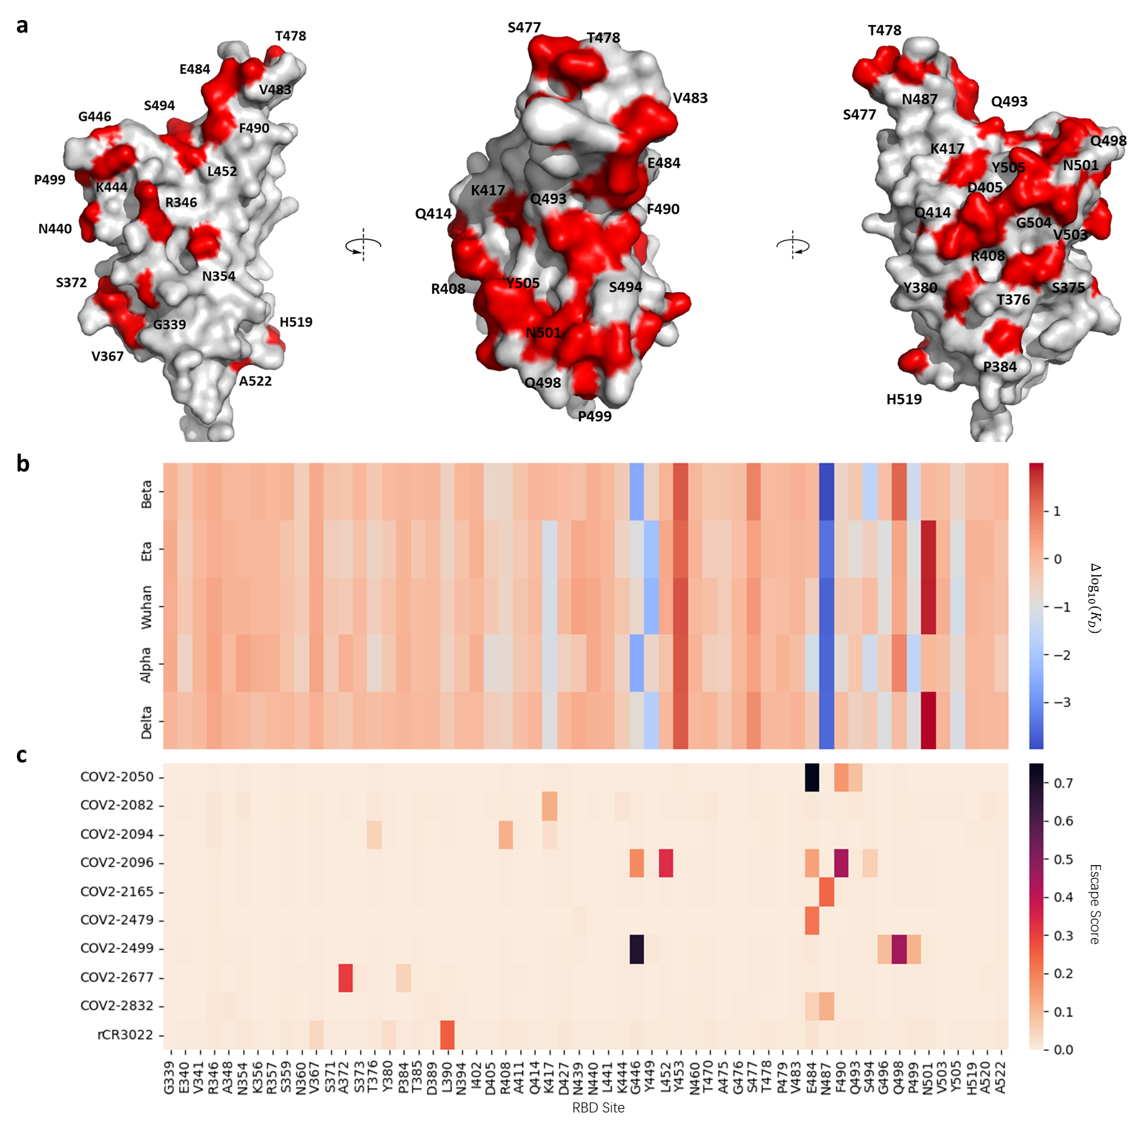
\includegraphics[width=1.0\linewidth]{figures/RBD Stucture.png}
	\captionsetup{justification=raggedright}
	\caption{Data analysis on deep mutational scanning from published work.\cite{starr_deep_2020}(a) 3D structure illustration of leading mutations outlined in RBD (red). (b) RBD-ACE2 binding affinity distribution with different reference virus variants. (c) Escape score of leading mutation sites.}
	\label{rbd-struc}
\end{figure}

Since the emergence of the first two reported variants, different SARS-CoV-2 variants have continued to acquire mutations in the RBD. Several of these RBD mutations were successfully outlined by our deLemus analysis. One such important mutation is N501Y, which appeared as a leading mutation in June 2020 in our deLemus analysis. This mutation can be found in the Alpha variant and the subsequent Beta, Gamma, Mu ($\mu$, B.1.621.1), and Omicron variants, as depicted in \fref{rbd}. Studies have shown that the N501Y mutation can enhance ACE2 binding affinity by introducing $\pi$-$\pi$ interactions between N501Y of RBD and Y41 of ACE2.\cite{Dejnirattisai2021} E484K is another notable mutation in the Beta variant that was outlined as a leading mutation from January 2020 by our deLemus analysis (\fref{rbd}). Mutations at this site have been demonstrated to significantly reduce the neutralization titers of convalescent plasma.\cite{Weisblum2020,Greaney2021,Baum2020} Although some studies have suggested that mutations of the E484 residue would lead to diminished electrostatic complementarity between the RBM and the ACE2 receptor,\cite{10.1038/s41467-022-28324-6} many structural biology studies have shown that the E484K mutation, when introduced with N501Y mutation, can increased RBD-ACE2 binding. For instance, in the Beta and Gamma variants, the E484K-N501Y-D614G triple mutation has been found to enhance RBD-ACE2 binding by inducing local rearrangements involving rotamer placements between Q493 of RBD and H34 of ACE2.\cite{Mannar2021}

Two other RBD mutations, L452R and T478K, were also outlined as leading mutations in April 2020 and November 2020 by our deLemus analysis (\fref{rbd}). These mutations were be found in the Delta variant that emerged in April 2021 (14\textsuperscript{th} month). Their locations within the epitope of several important neutralizing antibodies enable them to enhance the immune escape capabilities of the virus.\cite{Planas2021,Wang_mrna2021, li_impact_2020,Liu2021} For the L452R mutation, computational studies have shown that variants possessing the L452R-E484Q-N501Y triple mutation exhibit a secondary structure rearrangement that is associated with an increase in RBD-ACE2 binding affinity.\cite{10.1039/D1CP04005G} For the T478K mutation, structural analysis has revealed that it allows the formation of two new hydrogen bonds located between Y489 of RBD and Y83 of ACE2, and F490 of RBD and K31 of ACE2, respectively, resulting in tighter binding between the RBD and ACE2 receptor.\cite{10.1038/s41467-022-28528-w}

The Omicron variant that emerged in November 2021, known for its exceptionally high transmissibility, harbors a significant number of RBD mutations. Most of these mutations have been reported in previous variants, but several new sites were outlined as leading mutations by our deLemus analysis, which encompasses mutations at R408, N440, and G446. The R408S mutation has been shown to alter the antigenic property of the spike glycoprotein by disrupting the binding of F2 antibodies.\cite{Cao2022} Unlike R408S, the N440K mutation can enhance spike-ACE2 binding affinity by increasing the electrostatic complementarity between the structurally flexible RBM recognition site and the ACE2 receptor.\cite{Gan2021} As for the G446 residue, which is situated at a highly antigenic region of the spike structure (\fref{spike}), mutations have been shown to influence neutralization by both mAbs and antibodies present in polyclonal serum.\cite{li_impact_2020,starr_prospective_2021,Liu2021}

Overall, the leading mutations outlined within the RBD have been confirmed among the reported variants, suggesting their functional impact on viral fitness. Increased binding to the ACE2 receptor and immune evasion are factors that can enhance viral infectivity and overall viral fitness. \cite{Yi2022}
\cite{Mannar2021} These factors involve multiple amino acid residues located on the surface region of the spike protein. The spatial distribution analysis of the leading mutations highlights their prevalence on the surface region of the spike protein (\fref{rbd-struc}), which can enhance viral infectivity through host interactions, such as improved ACE2 binding affinity and antibody escape. This observation is further supported by previously reported deep mutational scanning data, which assesses ACE2 binding affinity and antibody escape scores.\cite{starr_deep_2020} 

\subsection{C-Terminal Domains (CTDs) and the S2 Subunit}

The post-RBD region of the SARS-CoV-2 spike glycoprotein consists of CTD1, CTD2, and the S2 subunit. While they do not directly engage the ACE2 receptor, they confer significant functions in spike allostery and membrane fusion.\cite{10.1126/science.abi6226, 10.1038/s41467-020-17371-6} The close spatial proximities between the CTDs and the NTD-RBD linker motif enable them to modulate RBD motion, and mutations in these regions could alter its open-close dynamics.\cite{Henderson2020, Gobeil2021, 10.1038/s41594-021-00652-z} The S2 mediates virus-host membrane fusion by undergoing a cascade of conformational changes,\cite{10.1073/pnas.2111199119, 10.1038/s41467-020-17371-6, 10.1038/s41580-021-00418-x} and its mutations may impact spike fusogenicity both in terms of host-virus membrane fusion for cell surface or endosomal entry and cell-cell membrane fusion for syncytia formation.\cite{10.1038/s41401-020-0485-4, 10.1038/s41580-021-00418-x} Additionally, the post-RBD region houses the S1/S2 and S2’ cleavage sites, which are proteolytically processed to facilitate membrane fusion.\cite{10.1038/s41580-021-00418-x, 10.1073/pnas.0809524106, Hoffman_multibasic2020, 10.1073/pnas.2111199119, Rajah2022} The former site is generated by a polybasic insertion between CTD2 and S2 (${}_{681}$PRRAR$\downarrow$S${}_{686}$) unique to SARS-CoV-2, and has been found to enhance its infectivity.\cite{Jaimes2020, Hoffman_multibasic2020, 10.1371/journal.ppat.1009246} Although their evolutionary importance is often overshadowed by those of the upstream NTD and RBD, the CTDs and S2 remain pivotal to the proper functioning of the spike.

\begin{figure}[!htbp]
	\centering
	\includegraphics[width=1.0\linewidth]{figures/Summary for CTD1-2.png}
	\captionsetup{justification=raggedright}
	\caption{Evolutionary trajectory of the C-terminal domains (CTD1 and CTD2). The annotations, labels, and color schemes in this figure are identical to those employed in \fref{ntd}.}
	\label{S12}
\end{figure}

The pre-alpha stage of the pandemic marked the phase in which several mutations hallmarked to the CTDs of later variants emerged. As shown in \fref{S12}, many of our CTD leading mutations outlined between January and December 2020 were reported in later VOCs and VOIs; these include: A570D, D614G, H655Y, Q677H, N679K, and P681H. One important leading mutation we outlined in the first month is D614G. It has been shown to promote RBD opening by disrupting an interprotomer hydrogen bond involving S2 residues,\cite{10.1016/j.celrep.2020.108630} and to increase S1/S2 cleavage, cell entry, replicative fitness, and transmissibility.\cite{10.1016/j.celrep.2020.108630, Ozono2021, Zhou2021} These enhancements in fitness led to its fixation in the global SARS-CoV-2 population. Most of the CTD mutations outlined above follow a similar trend in either finetuning RBD opening or cleavage efficiency. For example, A570D of Alpha has been revealed to form new interprotomer hydrogen bonds and salt-bridge interactions with S2 residues to modulate RBD motion.\cite{10.1126/science.abi6226, 10.1038/s41594-021-00652-z} Meanwhile, at the highly polymorphic P681 site, both P681H and P681R has been reported to increase S1/S2 cleavage efficiency.\cite{10.1016/j.isci.2021.103589, Saito2022, 10.1016/j.celrep.2022.110829} However, only P681R of Delta would have a pronounced effect in improving spike fusogenicity. \cite{10.1016/j.isci.2021.103589, Saito2022, 10.1016/j.celrep.2022.110829} Interestingly, the co-occurrence of N679K and P681H in Omicron variants has been found to introduce a novel cathepsin G cleavage site proximal to the S1/S2 furin cleavage site,\cite{10.1371/journal.pone.0264723} which may explain their switch from cell surface entry pathways preferred by pre-Omicron strains to endosomal entry pathways.\cite{10.1038/s41586-022-04474-x, 10.1038/s41392-022-00903-5, 10.1038/s41586-022-04479-6, 10.1038/s41564-022-01143-7, 10.1016/j.ebiom.2023.104753}

\begin{figure}[!htbp]
	\centering
	\includegraphics[width=1.0\linewidth]{figures/Summary for S2.png}
	\captionsetup{justification=raggedright}
	\caption{Evolutionary trajectory of the S2 subunit. The annotations, labels, and color schemes in this figure are identical to those employed in \fref{ntd}.}
	\label{S1b}
\end{figure}

Our deLemus method is also effective in outlining S2 mutations. As shown in \fref{S1b}, between January and December 2020, several outlined leading mutations of the S2 subunit were later confirmed in subsequent variants; these are: A701V, T716I, D796Y, S982A, D1118H, and V1176F. Unlike CTD mutations, the effects of the S2 mutations are more diverse.\cite{10.3390/v14030640} Both T716I and S982A of Alpha have been structurally determined to confer local destabilizing effect.\cite{10.1126/science.abi6226} In particular, the latter mutation has been shown to abrogate an interprotomer hydrogen bond with the CTD1 residue T547, which promotes RBD opening.\cite{10.1126/science.abi6226} In contrast, D1118H of Alpha has been suggested to impose stabilizing effects via water-mediated interactions.\cite{10.1038/s41421-021-00349-z} D796Y of Omicron, on the other hand, has been revealed to greatly enhance neutralization resistance and facilitate cross-domain immune evasion.\cite{10.1128/jvi.00922-23, 10.1128/spectrum.03291-23} As for V1176F of Gamma, it has been reported to reduce fusion activity of the spike.\cite{10.1073/pnas.2119467119} From January to November 2021, we also outlined multiple leading mutations that would later appear in the Delta and Omicron variants (\fref{S1b}); notably: N764K, N856K, T859N, D950N, Q954N, N969K, and L981F. Among these, N856K and N969K of Omicron have been shown to reduce fusion activity and syncytia formation,\cite{10.1016/j.celrep.2022.110729, 10.1038/s41392-022-01281-8, 10.1038/s42003-023-04923-x, 10.1080/22221751.2023.2297553} whereas D950N of Delta has been found to slightly promote membrane fusion.\cite{10.1016/j.ebiom.2023.104561}

To mitigate the global impacts of COVID-19, it is essential to strengthen worldwide surveillance systems for real-time monitoring and tracking of continuous mutations in SARS-CoV-2. In this study, we have developed a spike mutation tracking platform to monitor the evolutionary trajectories of spike glycoproteins (\href{https://hbsulab.github.io/deLemus/Updates/}{https://hbsulab.github.io/deLemus/Updates/}). This publicly accessible platform serves as an early warning system for upcoming variants, facilitating timely contributions in the ongoing efforts to combat SARS-CoV-2. The list of outlined leading mutations has been consistently updated on a monthly basis, extending beyond the 24-month timeframe discussed in the preceding sections. Any leading mutations that were subsequently confirmed in circulating variants would have been annotated and updated on the deLemus webpage. It is worth noting that certain mutations consistently appeared in our analysis. As shown in \fref{JN.1}, the persistent post-RBD mutations are: E554K, A570V, P621S, and S939F. These mutations would later be reported in the BA.2.86 lineage of Omicron which emerged in August 2023. This variant harbors over 30 new spike mutations when compared to the parental BA.2 strain.\cite{10.1136/bmj.p1964, 10.1016/S1473-3099(23)00575-3} Recent characterization has revealed that BA.2.86 shows improved ACE2-binding affinity,\cite{10.1038/s41586-023-06750-w} as well as enhanced immune escape capabilities due to its distinct antigenic profile.\cite{10.1016/S1473-3099(23)00573-X, 10.1016/S1473-3099(23)00575-3, 10.1016/j.vaccine.2023.10.051, 10.1038/s41467-023-43703-3} We also identified persistent mutations in the RBD region, namely K356T, R403K, and N450D, which are confirmed in BA.2.86 (\fref{JN.1}). Lastly, from the beginning of 2022, we observed a highly polymorphic site, L455, corresponding to the L455F/S mutations (\fref{JN.1}). In particular, L455S is a novel mutation carried by JN.1, a descendant lineage of BA.2.86, which emerged in December 2023. Remarkably, even though the two variants only differ by this single mutation, JN.1 has been demonstrated to exhibit even better immune evasion than BA.2.86.\cite{Yang2023, Yamasoba2023} This has likely enabled it to become the most prevalent strain globally since February 2024.\cite{WHO_jn1}

In addition to outlining the leading mutations, we revealed some general evolutionary features of the SARS-CoV-2 spike glycoprotein in terms of $\Xi$ and $\bm{\mathit{\bar{s}}}$. Mutations are the source of genetic variation, and how mutation rates fluctuate over the course of evolution is of particular interest.\cite{LYNCH2010345} Based on their $\Xi$ values, three characteristic evolutionary phases can be distinguished (Fig. S2). The first phase lasted from December 2019 to October 2020, when $\Xi$ maintained a steady state at relatively low values. In November 2020, a month before the emergence of Alpha, the second phase began with an increase of $\Xi$, to a maximum in March 2021, after which Delta appeared. This is followed by the third phase, marking the gradual decrease of $\Xi$ back to a steady state by June 2021. As most mutations are assumed to be neutral or slightly deleterious,\cite{10.1038/217624a0, 10.1038/246096a0, 10.1093/molbev/msi242} selection often acts against high mutation rates,\cite{10.1128/JVI.01031-17} which is illustrated by the initially low $\Xi$. This may also imply a dynamic equilibrium within the viral quasispecies,\cite{10.1016/0092-8674(78)90223-4, 10.1146/annurev.mi.41.100187.002205, 10.1128/mmbr.05023-11} where each pre-Alpha variant has similar fitness. The subsequent rise in $\Xi$ is thought to be a consequence of environmental changes,\cite{10.1128/mmbr.05023-11} which would increase the chances for beneficial mutations to occur.\cite{10.1128/JVI.01031-17} However, more deleterious mutations would likewise be introduced.\cite{10.1128/JVI.01031-17, 10.1073/pnas.1705887114} This may explain the resulting drop in $\Xi$. On the other hand, genetic diversity measured by $\bm{\mathit{\bar{s}}}$ exhibited a clear increasing trend from December 2019 (Fig. S2). This suggests the ongoing adaptive evolution of the spike,\cite{10.1038/nrg.2016.58} although further research would be required to elucidate the exact mechanisms that govern the complex evolutionary trajectory of SARS-CoV-2.

\begin{figure}[!htbp]
	\centering
	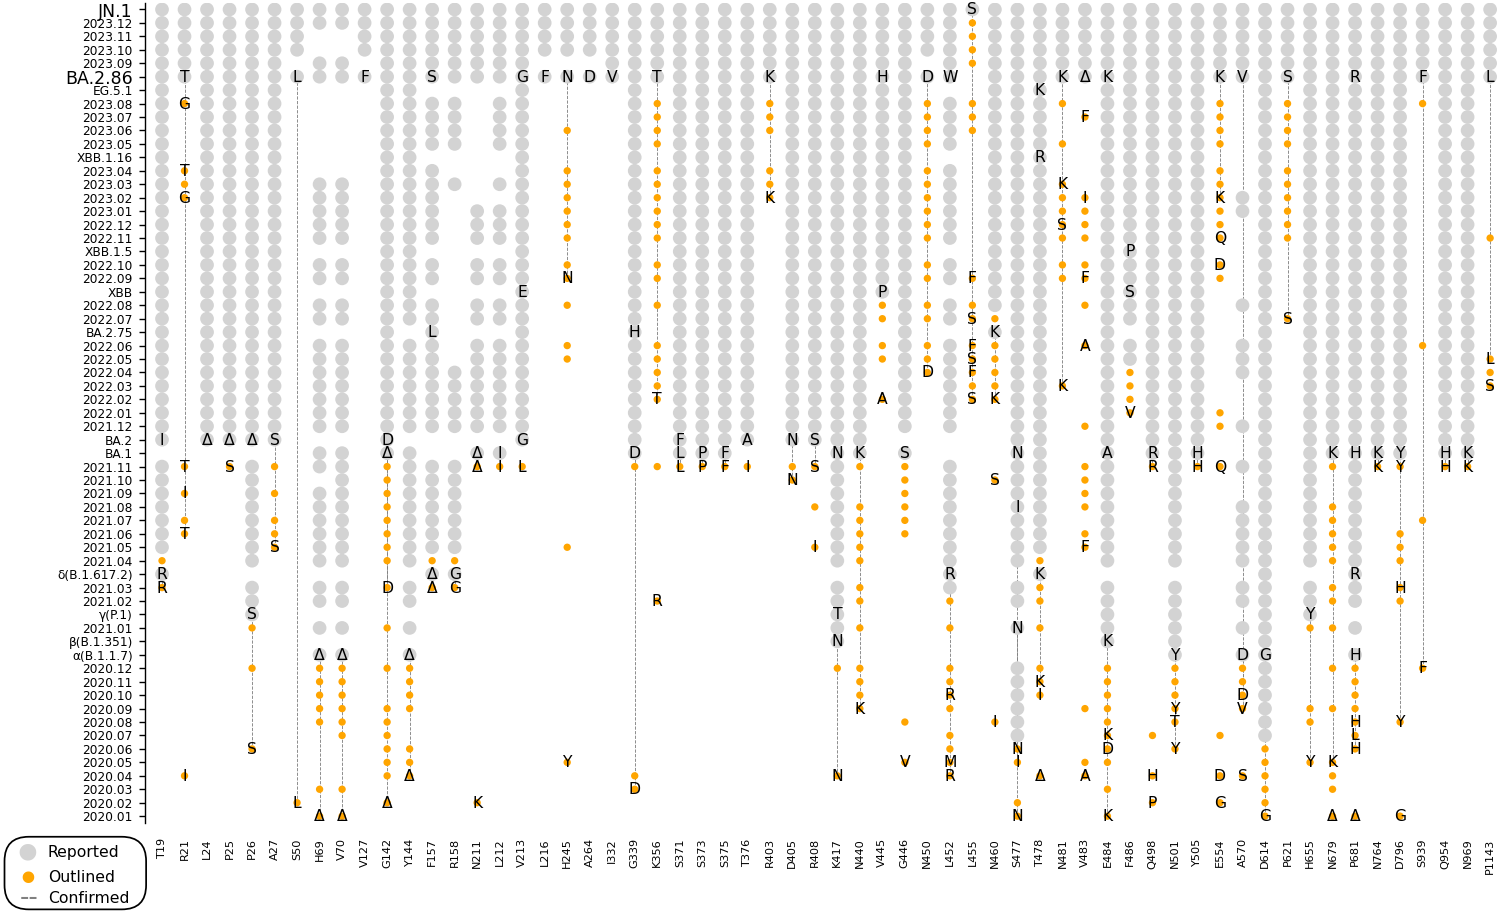
\includegraphics[width=1.0\linewidth]{figures/Summary for JN.1.png}
	\captionsetup{justification=raggedright}
	\caption{Evolutionary trajectory of the BA.2.86 and JN.1. The annotations, labels, and color schemes in this figure are identical to those employed in \fref{ntd}.}
	\label{JN.1}
\end{figure}

\section{Conclusion}

This work introduces the novel deLemus method for analyzing the evolutionary dynamics of the SARS-CoV-2 spike glycoprotein. Our proposed $\bm{L}$-index is effectual in quantifying the mutation strength of each amino acid site, such that leading mutations can be outlined (Table S2). Comprehensive characterization of these leading mutations reveals how the spike’s complex mutation pattern is shaped by the distinct evolutionary trajectory of each of its functional domains: the antigenic evolution of the NTD, the dynamic balance between ACE2-binding affinity and immune evasion by RBD mutations, and the cell entry mechanism shift modulated by post-RBD mutations. With its effectiveness in systematically monitoring the ongoing SARS-CoV-2 evolution, it may be feasible to extend our deLemus method to analyze other viral evolution processes. The ability to identify a subset of evolutionarily significant sites in circulating viruses would accelerate the development of treatments and disease control measures in the case of future pandemics.

\section{Data Availability}

All input data are freely available from GISAID. The code employed in this study is publicly accessible via the GitHub repository at \href{https://github.com/hbsulab/L-index.git}{https://github.com/hbsulab/L-index.git}. The results are available on the website and regularly updated on a monthly basis at \href{https://hbsulab.github.io/deLemus/}{https://hbsulab.github.io/deLemus/}. 

\section{Acknowledgements}
We acknowledge the data contributors and the GISAID Initiative for sharing the genetic sequence. We are grateful to Professor Yong Huang for many thought-provoking discussions and encouragement in the course of this work, which is supported in part by the Hong Kong Branch of South Marine Science and Engineering Guangdong Laboratory (SMSEGL20SC01) (for H.S.), ASPIRE League Partnership Seed Fund Program (ASPIRE 2019\#1), and Society of Interdisciplinary Research (SOIRÉE). This work has been funded by the Research Grants Council of Hong Kong (16305623) and HKUST grant (R9418). This research made use of the computing resources of the X-GPU cluster supported by the Hong Kong Research Grants Council Collaborative Research Fund (C6021-19EF). We would also like to acknowledge the enlightening advice from Jie Gao in the early stage of this work; the technical support from Long T. Ta and Siqi Lei for improving figures; and Ruichen Li, Leon R. Salim, and Salina Lam in data collection and preparation.

\newpage
\pagestyle{fancy}
\rhead{\thepage}
\lhead{}
\cfoot{}
\renewcommand{\headrulewidth}{0pt}
\printbibliography
\end{document}
